\chapter{Implementation of methods}
\label{cha:implementation_methods}
\hspace{10px}Although in the big data business there is a need to have more and more information (data), sometimes this is not always the best choice. It's true that a large amount of training data helps the machine learning model to learn more rules and generalize better to new data, however an undifferentiated addition of low quality data and input resources can introduce a lot of noise and at the same time, considerably slows down the training algorithm. In the presence of a data set with a large number of data columns, one should always question how many of these data features are actually informative for the model. If the number of features is equal to or greater than the number of observations stored in a data set, can lead a machine learning model to overfit. To avoid this type of problem, it is necessary to apply techniques that transform the data set to a reduced set of features that better represents the original data (Feature Extraction) or techniques that will estimate how informative each column is and, if necessary, remove it from the data set (Feature Selection).

Combining FS techniques with prediction and classification techniques has become a necessity in many applications \cite{LiuH} \cite{Elisseeff}. Feature selection has 3 major objectives, being: (1) avoid overfitting and improve model performance, i.e. higher prediction performance in the case of supervised classification and better cluster detection in the case of clustering; (2) provide faster and more cost-effective models; (3) gain a deeper insight into the underlying processes that generated the data. However, this advantages come at a certain cost, as the search for a subset of relevant features introduces a new layer of complexity in the modelling task. Instead of just optimizing the model parameters for the full feature set, we now need to find the optimal model parameters for the optimal feature subset, as there is no guarantee that the optimal parameters for the full feature set are equally optimal for the ideal subset of features \cite{Daelemans2003CombinedOO}. As a result, the search in the model's hypothesis space is amplified by another aspect: finding the optimal subset of relevant features. Feature selection techniques differ from each other in the way they incorporate feature selection search with the construction of the classification model.

On the other hand using FE creates new features based on the existing ones and then discarding the original features. It's a different type of feature reduction and also leads to other types of advantages such as: improvement in accuracy; reduction of overfitting risk; speed up in training; improvement in data visualization and increase in explainability of our model. These new reduced features set should be able to summarize most of the information contained in the original feature set. In this way, an abridged version of the original features can be created from a combination of the original set. The main difference between Feature Selection and Feature Extraction is that feature selection aims to rank the importance of the existing features in the data set and discard less important ones, no new features are created.

In this chapter, the steps taken to implement different feature selection and extraction techniques will be described in detail, as well as, understanding some of the results and conclusions that we can already deduce based on these algorithms. Principal Component Analysis (PCA), t-Distributed Stochastic Neighbor Embedding (t-SNE) and Linear Driscriminant Analysis (LDA) will be implemented as feature extraction algorithms and Chi-Square test (X), ANOVA F-test, Correlation Based Feature Selection (CFS) and Minimum Redundancy Maximum Relevance (MRMR) as feature selection algorithms. The results of these algorithms will later be used as input variables in classification algorithms such as deepDriver and Lotus to detect driver mutations based on the optimal subset of features previous selected. To have different mechanism to compare the results, these algorithms will be tested using 4 different data sets.

\section{Feature Extraction methods} % (fold)
\label{sec:feature_selection}

\subsection{PCA - Principal Component Analysis} % (fold)
\label{sec:pca}
\hspace{10px}Principal component analysis (PCA) is one of the most used linear dimensionality reduction technique. It's a statistical procedure that orthogonally transforms the original n numeric dimensions of a data set into a new set of m dimensions called principal components, where m<n. As a result of the transformation, the first principal component has the largest possible variance and each succeeding principal component has the highest possible variance under the constraint that it is uncorrelated with the preceding principal components. Keeping only the first m principal components reduces the data dimensionality and at the same time retains most of the information in the data.

One of the ways to implement this method would be by computing the \textit{eigenvectors} and corresponding \textit{eigenvalues} of the covariance matrix. The \textit{eigenvalues} are used to sort the \textit{eigenvectors} in order to give us the principal components in order of importance. The larger the \textit{eigenvalues}, the more important that principal component is. This article, \href{https://sebastianraschka.com/Articles/2014_pca_step_by_step.html#1-taking-the-whole-dataset-ignoring-the-class-labels}{here}, gives a good explanation on how to implement PCA using this method.

The other way, and this is the one that will be used because it is simpler and faster to implement, would be to use the Scikit-Learn implementation of PCA. Another thing that it's possible to test with this library, is the cumulative explained variance based on the number of components, the figure \ref{fig:variance_graph} illustrates this relation. 

\begin{figure}[h]
    \centering
    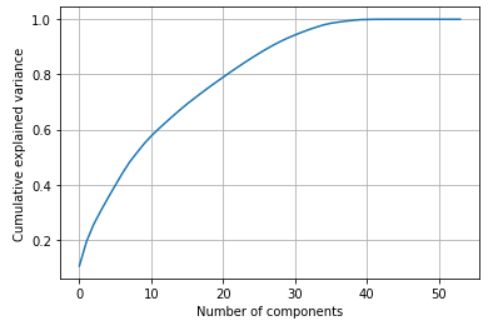
\includegraphics[width=0.6\textwidth,height=0.2\textheight]{Chapters/Figures/number_of_components.png}
    \caption{Cumulative Explained Variance\\ as a function of the Number of Components}
    \label{fig:variance_graph}
\end{figure}

As we can see, to achieve at least 90\% of information it's needed at least 30 components aka features. This was tested with various data sets and the results was always the same, minimum of 30 components to achieve 90\% of information the biggest difference being the slope of the curve were some have less cumulative explained variance with less components. Since we as humans being, can only view and perceive things in two- or three-dimensions, from the original 48 dimensions we chose only the the first three principal components.

First PCA will be performed in the whole data set to reduce the data to just two dimensions and then construct a data frame with these new features and their respective labels, like so:

\begin{lstlisting}[language=Python]
def PCA_algorithm(X):
    n_components=2
    pca = PCA(n_components)

    X_pca = pca.fit_transform(X)
    columns = []
    i=1
    while i <= n_components:
        columns.append("PC"+str(i))
        i+=1
    PCA_df = pd.DataFrame(data = X_pca, columns=columns)
return PCA_df
\end{lstlisting}

These two component represent 18.35\% of total variance explained with 0.16047499 as a variance for the first component and 0.12055106 for the second component. Even so, these values leave a lot to be desired when faced with larger data sets, where increasing the number of rows and maintaining the same level of information causes significant loss of variance, the next data set had a 14.3\% of total variance explained the second had 19.27\%, and the last one around 20\%. 


\begin{figure}[h]
    \centering
    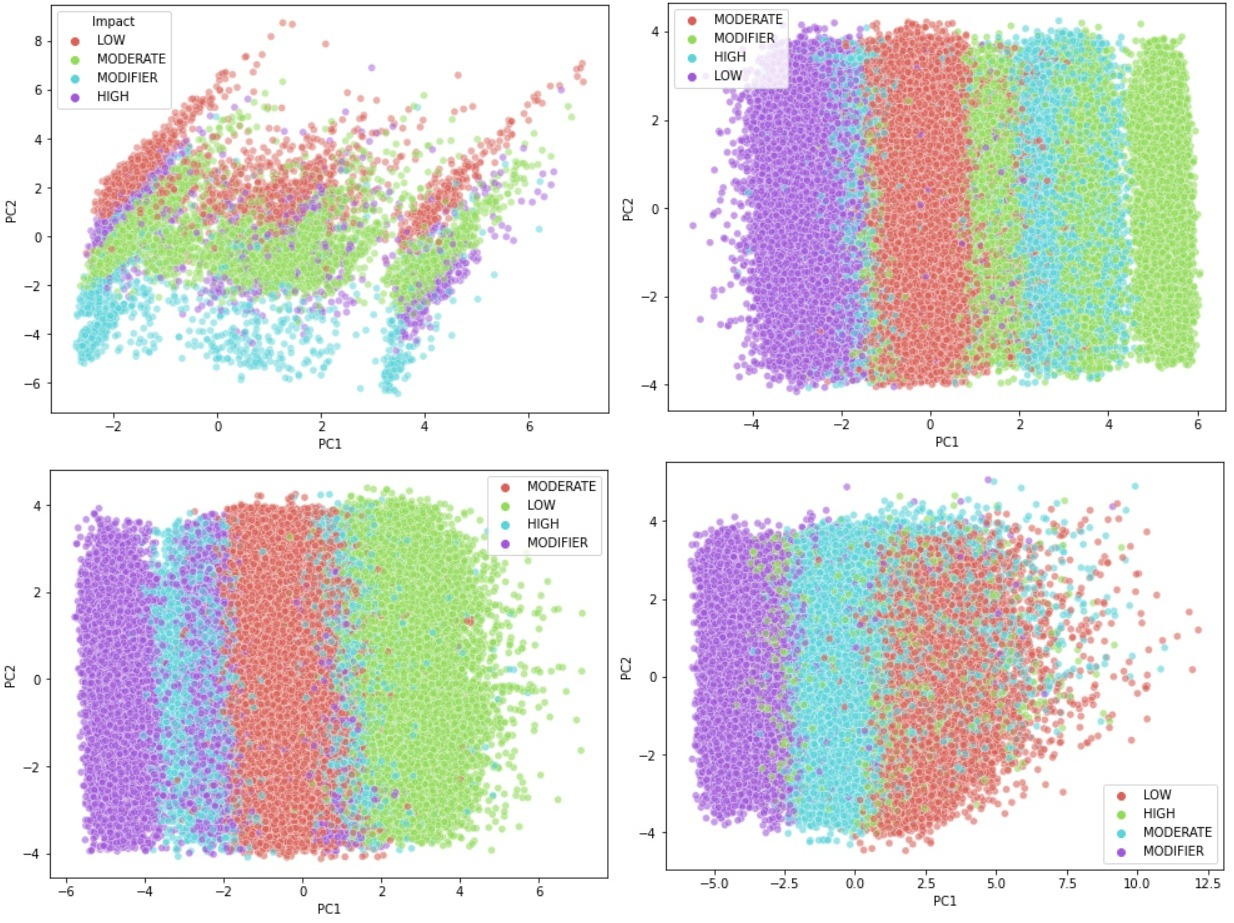
\includegraphics[width=0.9\textwidth,height=0.35\textheight]{Chapters/Figures/pca4.jpg}
    \caption{2D PCA Graph using 4 different data sets}
    \label{fig:pca_graph}
\end{figure}

The graphs above show the relationship of the two main components (PC1 and PC2) with the Impact target variable using four different data sets. Although there are significant and visible differences in each graph, they share some similarities such as having an order in the distribution of the variables, some are being overlapped by other variables and the variables with HIGH Impact are barely visible or almost non-existent compared to the remaining variables, where clusters of the remaining types of Impact categories are visible. To fight for better representation and visualization of the data, a 3d version of each graph was created where it is possible to select which category(ies) one wants to visualize and analyze. It's possible to view it later here (reference to my git hub).

Re-running the Random Forest Classifier but this time using this set of 2 features built by the PCA led to 82\% classification accuracy while using 3 features lead to 90\% of accuracy, this for the first data set. The other data sets, as they present much higher dimensions, for example the fourth data set used has approximately 13x more information than the first data set, which leads to a decrease in classification accuracy, with only two features it has 75\% of classification accuracy, mean while with 3 features has 88\% of classification accuracy.


\subsection{t-SNE} % (fold)
\label{sec:tsne}
\hspace{10px}A lot has changed in the world of data science since the development of PCA in 1933, mainly in the realm of compute and size of data. t-distributed Stochastic Neighbor Embedding (t-SNE) first developed by Laurens van der Maatens and Geoffrey Hinton in 2008, it's an unsupervised, non-linear dimensionality reduction technique primarily used for data exploration and is well suited for the visualization of high-dimensional datasets. It gives a sense or intuition of how data is organized in a high-dimensional space \cite{Laurens}. Being a non-linear dimensionality reduction technique allows to separate data that cannot be separated by any straight line like: cylinder, ball, curve, etc. t-SNE differs from PCA by preserving only small pairwise distances or local similarities. This becomes a great advantage, unlike PCA, which being a linear dimension reduction technique, seeks to maximize the variance while preserving large distances between the pairs, it means that different things end up distant which can lead to a worse visualization, especially when it comes to structures of nonlinear manifolds.

The t-SNE algorithm works by calculating a similarity measure between pairs of instances in high dimensional space and in low dimensional space and then tries to optimize these two similarity measures using a cost function. It has 3 major steps: First, it measure similarities between points in the high dimensional space. For each data point, a Gaussian distribution will be centered. Then measure the density of all points under this Gaussian distribution and finally renormalize for all points. What this does is create a set of probabilities for all points. These probabilities are proportional to the similarities, which means that if two data points have equal values under this Gaussian circle, their proportions and similarities are equal, and therefore there are local similarities in the structure of this high-dimensional space. Using the perplexity parameter it is possible to manipulate the Gaussian circle, which in turn influences the variation of the distribution (circle size) and at the same time influences the number of  of nearest neighbors. The normal range for perplexity is between 5 and 50 \cite{scikit-learn}. Second, similar to the first step, the only difference is that it uses a Student's t distribution with one degree of freedom, also known as the Cauchy distribution. The Student's t-distribution has heavier tail than the normal distribution, which allows for better modeling of large distances. This distribution provides a second set of probabilities in low-dimensional space. Third, the set of probabilities of the low-dimensional space must reflect, as best as possible, those of the high-dimensional space. In order for the two map structures to be similar, the difference between the probability distributions of the two-dimensional spaces is measured using the Kullback-Liebler divergence (KL). It is an asymmetric approach that efficiently compares high probability values with low probability values. Finally, a gradient descent is used to minimize the cost of the KL function.

\begin{lstlisting}[language=Python]
def tSNE_algorithm(X):
    time_start = time.time()
    perplexity = int(pow(len(X) ,1/2))
    tsne = TSNE(n_components=2, verbose=1, perplexity=perplexity)
    
    tsne_results = tsne.fit_transform(X)
    
    print("t-SNE_done!_Time_elapsed:_{}_seconds"
    .format(time.time()-time_start))
    
    tsne_df = pd.DataFrame(data = tsne_results,
    columns=["tsne-1","tsne-2"])
    
    tsne_df = pd.concat([tsne_df, table["IMPACT"]], axis = 1)

return tsne_df
\end{lstlisting}

Above is the implementation of the t-SNE algorithm using the implementation available at the Scikit-Learn documentation \cite{scikit-learn}. Typical perplexity has it's values range between 5 and 50. But according to \cite{wattenberg2016how} the optimal value for perplexity for any particular data set is calculated from the number of cells according to the power law Perplexity \(\cong N^\frac{1}{2}\), so perplexity is calculated by \textbf{int(pow(len(X)} ,1/2)). This power law is very similar to the rule of thumb for selecting optimal K in the K - Nearest Neighbors (KNN) algorithm.  

\begin{figure}[h]
    \centering
    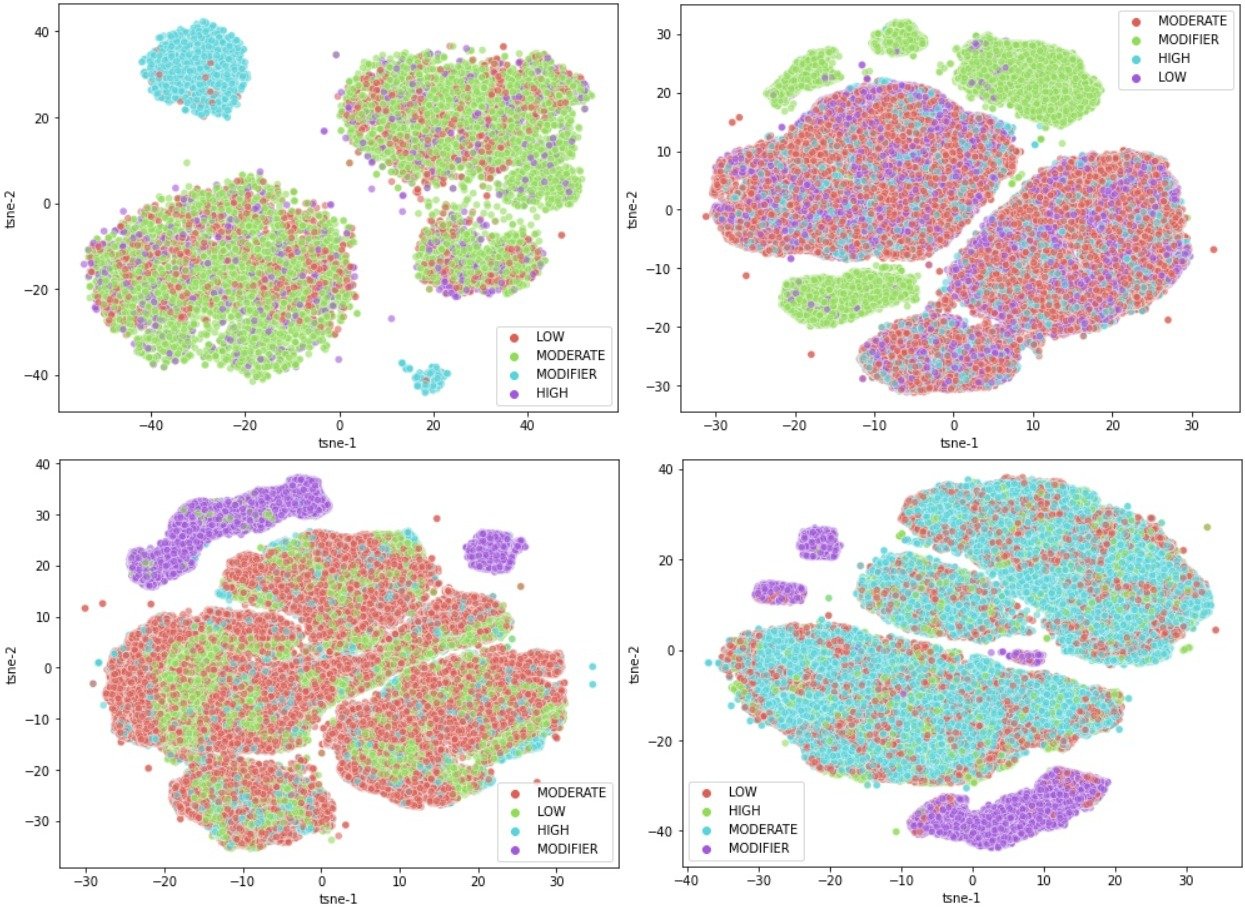
\includegraphics[width=0.9\textwidth,height=0.35\textheight]{Chapters/Figures/tsne4.1.jpg}
    \caption{2D t-SNE Graph using 4 different data sets}
    \label{fig:tsne_graph}
\end{figure}

Viewing the distribution of the resulting features in Fig.\ref{fig:tsne_graph}, we can clearly see how well our data was separated even though it was transformed into a small space. Although this technique uses fewer dimensions by combining both distributions, the way in which this is done is computationally quite heavy so there are some (serious) limitations to using this technique. One of the limitations is in the presence of very high dimensional data, it may be necessary to apply another dimensionality reduction technique before using t-SNE, in this case it is not necessary because the data sets are previously reduced to less than 50 features in the data preprocessing. The other limitation that proved to be more challenging is that t-SNE scales quadratically on the number of objects N, which makes its use limited to datasets with only a few thousand input objects, for higher values learning becomes too slow to be practical and memory requirements become too high.

\subsection{LDA - Linear Driscriminant Analysis} % (fold)
\label{sec:lda}
\hspace{10px}Linear Discriminant Analysis (LDA) was first introduced in 1936 as Fisher's linear discriminant, a method used in statistics to find a linear combination of features that characterizes or separates two classes of objects, later being generalized to several classes in 1948 by C.R. Rao. It is a supervised learning dimensionality reduction technique as well as a machine learning classifier. Then after applying the algorithm for feature reduction, LDA will be used as a classifier in the results to evaluate the performance of dimension reduction.

To project data from a D dimensional feature space down to a D’ dimensional space where D'< D, LDA aims to maximize the distance between the mean of each class and at the same time minimize the spread within the class itself. This is a good decision because maximizing the distance between the means of each class and projecting the data into a smaller dimensional space leads to better classification results \cite{Pier}. Similar to the ANOVA test in feature selection, the LDA algorithm has some requirements to fulfill: input data must follow a Gaussian Distribution (not using a Gaussian data can lead to poor classification results) and each input variable has the same variance, so it's best to to standardize the data before using LDA.

\begin{lstlisting}[language=Python]
#normalize data 
norml_data = PowerTransformer(method="yeo-johnson",standardize=True)
            .fit_transform(X)

lda = LinearDiscriminantAnalysis(n_components=2)
X_lda = lda.fit_transform(norml_data, Y)

# Calculate the variance explained by priciple components
print("Variance of each component:", lda.explained_variance_ratio_)
print("Total Variance Explained:", 
      round(sum(list(lda.explained_variance_ratio_))*100, 2))
\end{lstlisting}

To transform the data to make more Gaussian-like, the scikit-learn library has a built in function in \textit{sklearn.preprocessing.PowerTransformer} that transforms data using the Box-Cox transformation or the Yeo-Johnson transformation. Box-Cox requires the input data to be strictly positive, while Yeo-Johnson supports both positive and negative data and since the data has both positive and negative values, the method used is Yeo-Johnson. Setting standardize to True applies unit variance normalization to the transformed output.
After that, all that remains is to apply the LDA algorithm, also present in the scikit-learn library, with only 2 components. Below are the 2D graphics of the dataset after using the LDA, where one can clearly see the mutations being clustered with great precision based on their impact category.

\begin{figure}[h]
    \centering
    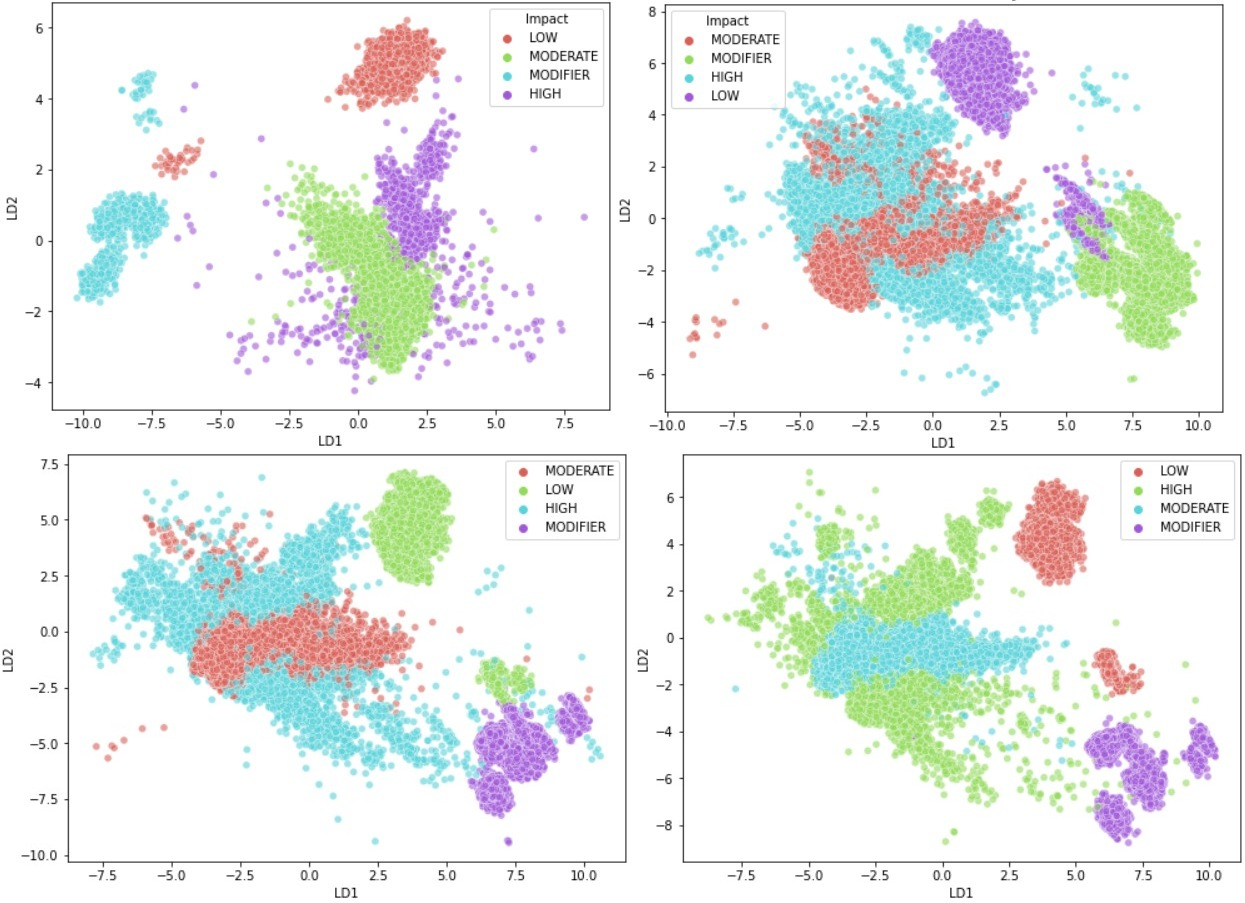
\includegraphics[width=0.9\textwidth,height=0.35\textheight]{Chapters/Figures/lda4.jpg}
    \caption{2D LDA Graph using 4 different data sets}
    \label{fig:lda_graph}
\end{figure}

The explain variance with only two features reached values over 90\% with some reaching 100\% when using three features. These results were quite promising as they also achieved high results of accuracy in both classification test (forest test and LDA test) with the 4 data sets having over 90\% accuracy with only two components or features. Of the three feature extraction techniques, LDA has proven to be the most accurate algorithm in representing the original data, the fastest to execute and the least cost in time and memory.

\section{Feature Selection methods} % (fold)
\label{sec:feature_extraction}
\hspace{10px}Now, lets move on to the implementation of feature selection algorithms. Unlike FE, FS reduces the number of features by discarding all but the best. This process can be done on three different occasions: when examining and discarding features before the classifier training process; when using the performance of a training hypothesis; by embedding the selection within the classifier construction. For reasons of simplicity, easy understanding and use of the code in future works and researches, it was decided to implement algorithms that make the selection before the classifier training process. This selection is called filtering and can be univariate filtering if features are discarded when examining each feature individually, or multivariate filtering if features are analyzed together with other features.

Filtering techniques assess the relevance of features by looking only at the specific properties of the data. These techniques are easily scaled to large datasets, are computationally simple and fast, and are independent of the classification algorithm. Therefore, the selection of features only needs to be performed once before applying different classifiers.


\subsection{Univariate Filtering} % (fold)
\label{sec:inserting_tables}

\subsubsection{Chi-Square test} % (fold)
\label{sec:inserting_tables}
\hspace{10px} One of the criteria to select the best features, which is given by the Chi-Square test (\(X^2\)), would be to eliminate the features that are statistically independent of the class, since they are considered as noise and are useless to predict the class. Furthermore, this test allows us to perceive the relationship between categorical variables of the data set, that is, it helps to find correlations between different categorical variables. 
Before performing the chi-square test, it is necessary to initially consider 2 hypotheses: the Null Hypothesis and the Alternative Hypothesis. The null hypothesis can be structured as follows: The cluster variables have no association or correlation with each other. The alternative hypothesis goes as follows: The variables are associated with each other and have a correlation between the variables.

The easiest and best way to implement chi-square test in python is to use chi2 function from sklearn.feature\_selection library\cite{scikit-learn}. The function takes 2 parameters which are: X - sample vectors, our data set (n\_samples,n\_features) and Y - target vector or class label (n\_samples). This function returns 2 arrays, the first array contains the chi2 statistics and the second the p\_values. The p\_values are the values that determine the dependency of the variables. If the p value is less than 0.05 the null hypothesis is rejected and the alternative hypothesis is accepted and if the p value is greater than 0.05 the null hypothesis is accepted and the alternative hypothesis is rejected.

\begin{lstlisting}[language=Python]
#chi-square test 
chi_scores = chi2(X,Y)

#retrieve p_values from chi_scores and plot the results
p_values = pd.Series(chi_scores[1],index = X.columns)
p_values.sort_values(ascending = False , inplace = True)
p_values.plot.bar()

#remove features with p_value grater than 0.05
to_remove = []
for index, value in p_values.items():
    if value > 0.05:
        to_remove.append(index)
best_features = X.drop(to_remove,axis=1)
\end{lstlisting}

\begin{figure}[h]
    \centering
    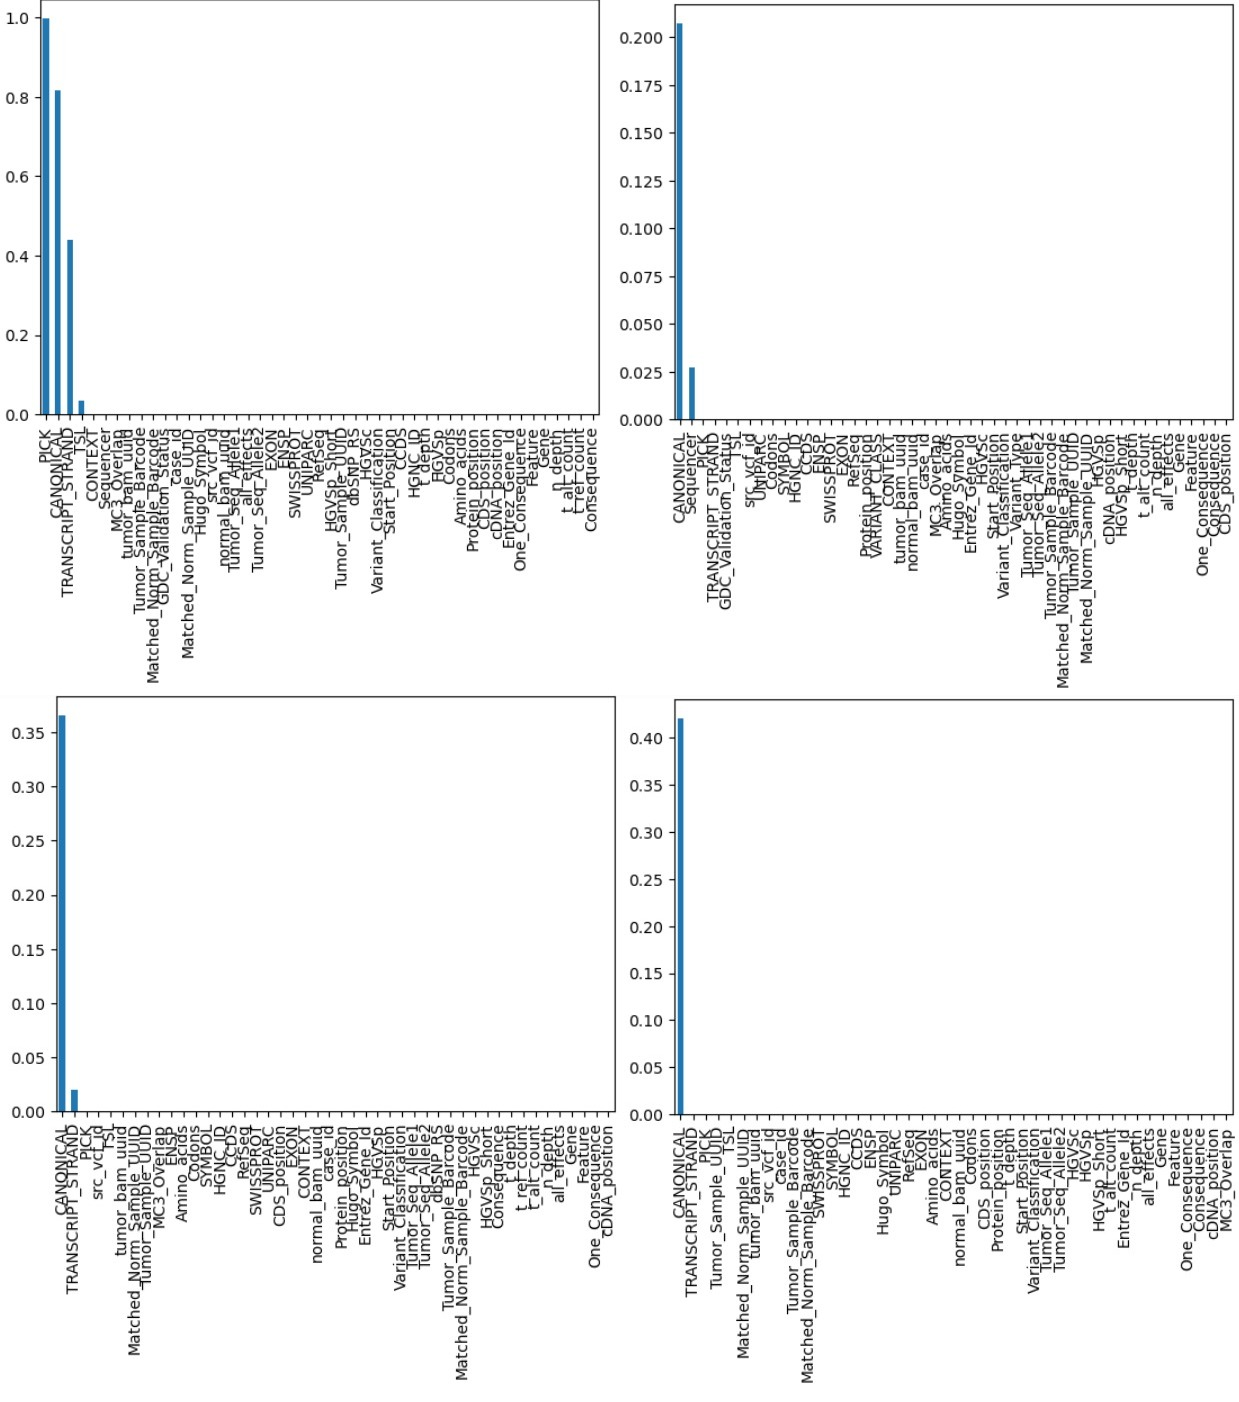
\includegraphics[width=0.95\textwidth,height=0.55\textheight]{Chapters/Figures/chi_square_test.jpg}
    \caption{p\_value of features in 4 different data sets}
    \label{fig:chi_graph}
\end{figure}

The graphs above show the p\_value values for each feature in 4 different data sets. Not all graphs have the same number of features to be removed (features with p\_value > 0.05) but they all agree on removing ate least one feature, the CANONICAL feature.

\begin{lstlisting}[language=Python]
#select the top k features
selected_features = SelectKBest(chi2,k=7).fit(X,Y)
best_columns = X.columns[selected_features.get_support()]
best_features = X[best_columns]
best_features
\end{lstlisting}

To select the best features, the more significant ones, they must have the lowest P value possible. SelectKBest is a builtin function in sklearn.feature\_selection that selects the best k features according to the scoring metric provided. The scoring metric passed is chi2 and k = 7 features. Then use the fit method to fit the current data set and get the name of selected columns. Finally, the resulting data set is tested with the forest\_test and achieved 0.96 in accuracy. More features only increased the accuracy and with 10 features achieved 1.00 in accuracy.

\subsubsection{ANOVA F-test} % (fold)
\label{sec:inserting_tables}
\hspace{10px} Another criterion would be to compare the means of each group of the independent categorical variable, that is, to estimate the extent to which a dependent variable is affected by one or more independent categorical data elements. This estimate is given by the ANOVA F-test, it is a statistical test that can say whether an independent variable has a significant influence on the dependent variable.

However, the results of this test become invalid if certain requirements are not met. ANOVA assumes that the variables are independent of each other and that the variables follow a Gaussian distribution. In this case the sample data is obtained independently and randomly from the population and it is possible to test whether the data follows a normal distribution by using histograms, skewness and kurtosis values, or using tests such as Shapiro-Wilk or Kolmogorov-Smirnov. Fig.\ref{fig:histogram} shows the frequency distribution of one of the data sets on the left and on the right, the same data set after a transformation to normal has been performed. It is easy to conclude that the data do not follow a Gaussian distribution, being necessary to transform them to a distribution more similar to the normal distribution (this test was done in several data sets and none of them follows a normal distribution, which makes it mandatory to do this transformation before using this algorithm). Again, as was done before in the LDA test, a PowerTransformer will be implemented in the data set and as a parameter, yeo-johnson is provided as the transform to use.

\begin{figure}[h]
    \centering
    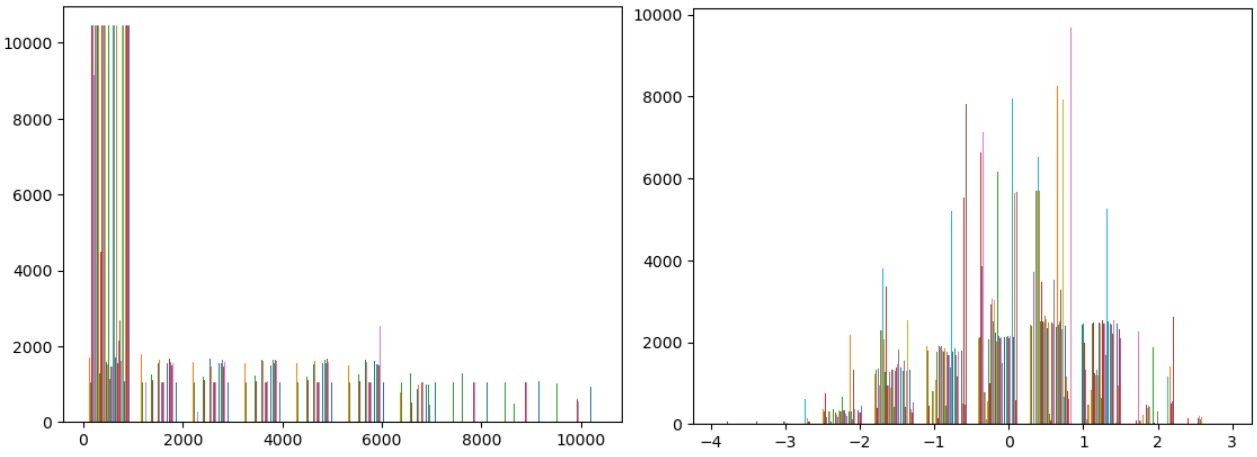
\includegraphics[width=0.6\textwidth,height=0.15\textheight]{Chapters/Figures/hist_norm.jpg}
    \caption{p\_value of features in 4 different data sets}
    \label{fig:histogram}
\end{figure}

To perform any test, it is necessary to define two hypotheses the null hypothesis and the alternative hypothesis. Null hypothesis: there is no significant difference between the groups. Alternative Hypothesis: There is a significant difference between the groups. Basically, ANOVA is performed by comparing two types of variation, the variation between the means of the groups and the variation within each one of the groups. The code below shows how to implement the ANOVA F-test using the Scikit-Learn library.

The result of the F-test allows us to analyze which features deviate the most from being class-independent and and are those that have the lowest probability value. If the p-value is smaller than 0.05, then the null hypothesis is rejected and the alternative hypothesis is supported.

\begin{lstlisting}[language=Python]

#ANOVA F-test test
univariate_f = f_classif(X,Y)
univariate_funivariate = pd.Series(univariate_f[1],index = X.columns)
univariate.sort_values(ascending = False , inplace = True)
univariate.plot.bar()

#remove features with p_value grater than 0.05
to_remove = []
for index, value in univariate.items():
    if value > 0.05:
        to_remove.append(index)
best_features = X.drop(to_remove,axis=1)
\end{lstlisting}

The graphs bellow show the p\_value values for each feature in 4 different data sets. The higher the P Value the lesser the importance of this feature. The features with p-value greater than 0.05 will be removed of the data set.

\begin{figure}[h]
    \centering
    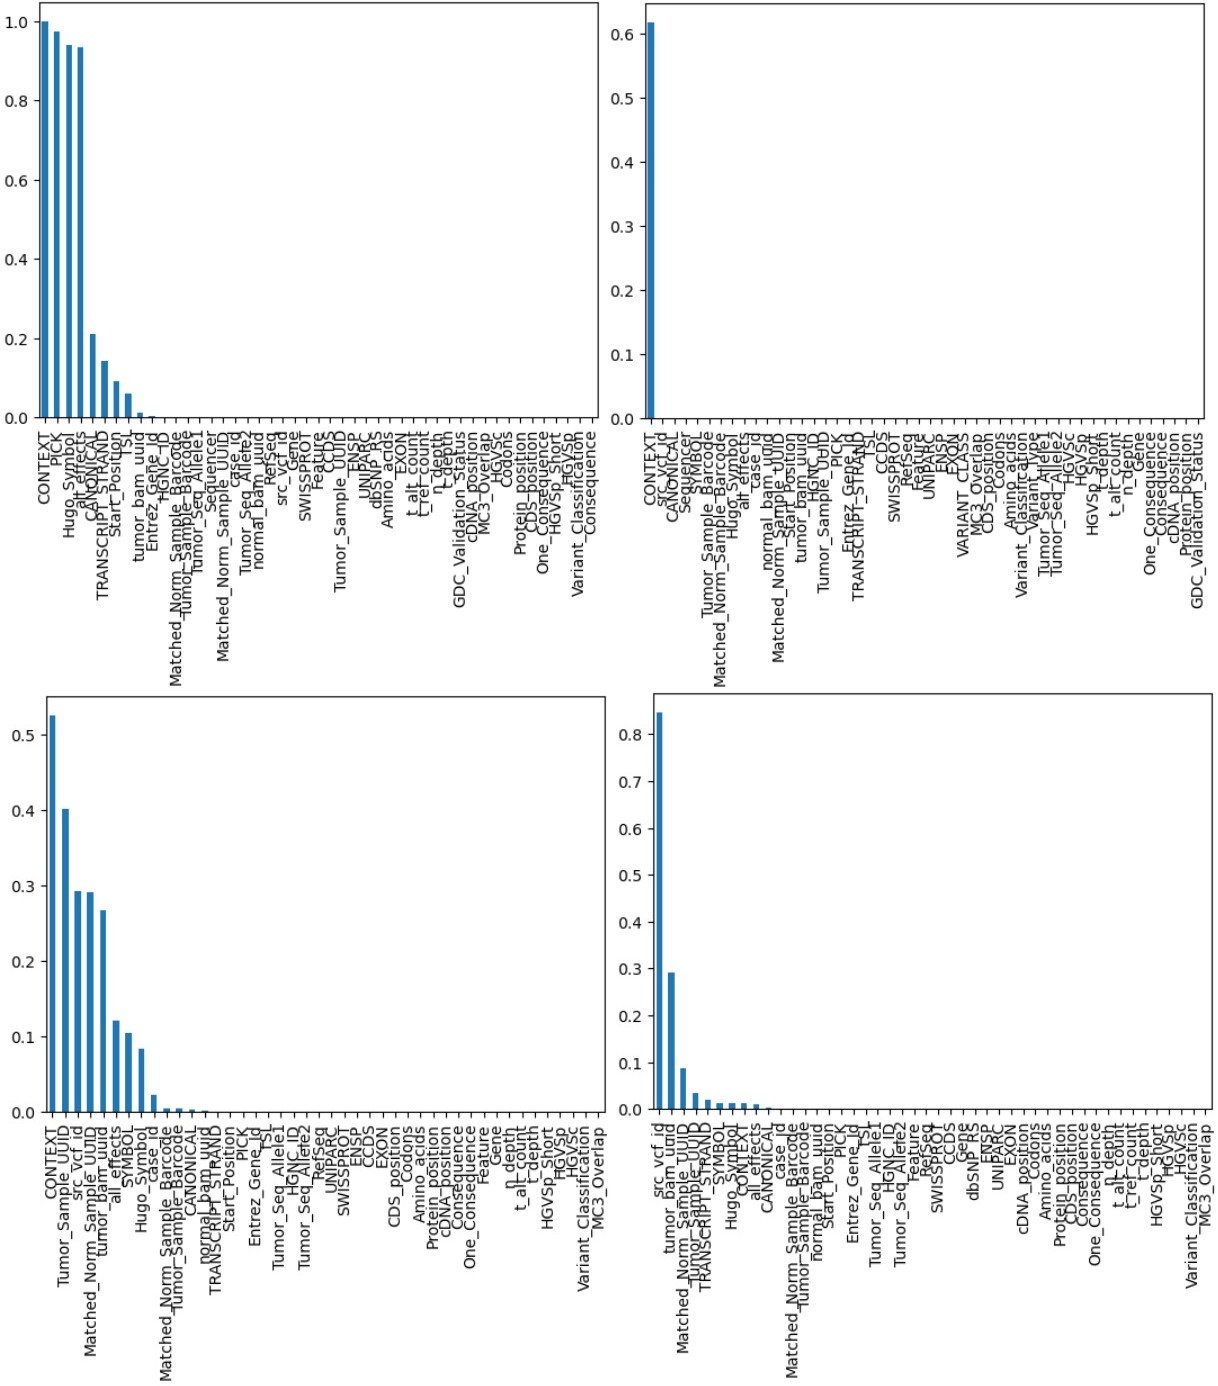
\includegraphics[width=0.95\textwidth,height=0.55\textheight]{Chapters/Figures/anova_test.jpg}
    \caption{ANOVA F-test in 4 different data sets}
    \label{fig:lda_graph}
\end{figure}

To select the best features, the more significant ones, they must have the lowest P value possible. Once again the function SelectKBest provided by sklearn.feature\_selection, selects the best k features according to the scoring metric provided. The scoring metric passed, this time, is f\_classif and k = 10 features. Then use the fit method to fit the current data set and get the name of selected columns. Finally, the resulting data set is tested with the forest\_test and achieved 1.00 (100\%) accuracy with only 10 features, the same value was achieved initially with 48 features.


\begin{lstlisting}[language=Python]
#select the top k features
selected_features = SelectKBest(f_classif,k=10).fit(X,Y)
best_columns = X.columns[selected_features.get_support()]
best_features = X[best_columns]
best_features
\end{lstlisting}



\subsection{Multivariate Filtering} % (fold)
\label{sec:inserting_tables}

\subsubsection{CFS – Correlation Based Feature Selection} 
\label{sec:inserting_tables}
\hspace{10px}Correlation is a statistical term used to describe the degree to which two variables move in coordination with each other. For example, one variable can cause or depend on the values of another variable, it can be loosely associated with another variable, or even two variables can depend on a third unknown variable.  It is a very useful filtering method in data analysis and modeling to better understand the relationships between variables. There are 3 types of correlation: positive correlation both variables move in the same direction; negative correlation variables change in opposite directions, that is, when the value of one variable increases, the values of the other variables decrease; Neutral correlation means that the variables have no relationship between variables. The type of correlation of the variables is provided by the correlation coefficient. It takes values between -1 and 1. Values close to 0 imply a weak correlation and exactly 0 means that there is no correlation between variables. Values close to 1 mean that there is a strong positive correlation between the variables and values close to -1 means that there is a strong negative correlation between the variables.

In this work the focus will be on the correlation between the input variables (features) with the target variable ("Impact") to provide information about which variables may or may not be relevant as input for the development of a classifier. For this, only the features with the correlation coefficient value above 0.5 will be chosen. The correlation coefficient values are provided by the correlation matrix, it consists of a table (rows and columns) in which each cell contains the correlation coefficient between all possible pairs of values. It is a powerful tool, provided by the Pandas library, and serves to summarize large datasets and identify and visualize patterns in the same data.


There are 3 techniques for calculating the correlation of variables, Pearson Correlation, Spearman Correlation, and Kendall Correlation. The use of one of these techniques will depend on certain assumptions that the data set has to fulfill. For example, the use of Pearson Correlation implies that the data follows a normal distribution (which we have already seen is not the case), the presence of outliers can interfere with the results of the algorithm and the data has to follow a line (linear data). The advantage of Spearman Correlation is that it does not depend on the normality of the data and does not require the data to follow a linear relationship. However, the Kendall correlation has very different results from the other two, because Kendall is more of a dependency strength test that measures a linear dependence between two variables \cite{Hall}. That said, Spearman Correlation was chosen for implementation.

Below is the Pearson correlation implementation code and using a heatmap it is possible to see the correlations between the independent variables and the target variable.

\begin{lstlisting}[language=Python]
target = pd.Series(Y, name="Impact")
new_X = pd.concat([X,target], axis = 1)

#Using Spearman Correlation
plt.figure(figsize=(20,16))
cor = new_X.corr(method="spearman")
sns.heatmap(cor, annot=True, cmap=plt.cm.Reds)
plt.show()

#Correlation with target variable
cor_target = abs(cor["Impact"])

#Selecting highly correlated features
corr_features = cor_target[cor_target>0.5]
\end{lstlisting}

\begin{figure}[h]
    \centering
    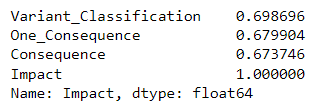
\includegraphics[width=0.55\textwidth,height=0.1\textheight]{Chapters/Figures/cfs.png}
    \caption{Highly correlated features}
    \label{fig:lda_graph}
\end{figure}

As you can see, only the Variant\_Classification, One\_Consequence and Consequence features are highly correlated with the target variable IMPACT. Therefore, all other features except these will be discarded. Another assumption is that the independent variables have to be uncorrelated with each other. So, if there are variables correlated with each other, only one of them is needed and the rest are discarded. This verification can be done visually on the correlation matrix plot or by the explicit code below.

\begin{lstlisting}[language=Python]
#keep features with high correlation
best_features = new_X[corr_features.index]

print(new_X[["Variant_Classification","One_Consequence"]].corr())
print(new_X[["One_Consequence","Consequence"]].corr())

\end{lstlisting}


\begin{figure}[h]
    \centering
    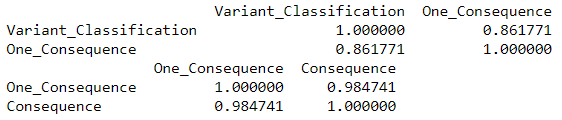
\includegraphics[width=0.65\textwidth,height=0.1\textheight]{Chapters/Figures/cfs_1.png}
    \caption{Highly correlated features}
    \label{fig:lda_graph}
\end{figure}

The code above allows to conclude that Variant\_Classification and One\_Consequence and One\_Consequence and Consequence are highly correlated with each other with 0.861 and 0.984 respectively. Therefore, only one of the variables would be kept and the others will be discarded. The Variant\_Classification will be the only one to keep, since it is the one with the highest correlation of the 3.


\subsubsection{MRMR – Minimum Redundancy Maximum Relevance}
\label{sec:inserting_tables}
\hspace{10px} MRMR, acronym for Maximum Relevance — Minimum Redundancy, first devised and published in 2005 by two Berkeley researchers \cite{Ding}, gained popularity again after this \cite{Zhenyu} article was published in 2019 by Uber engineers. In 2005 it was proved that genes selected using this technique have been shown to provide more balanced coverage of space and capture broader features of phenotypes. It was tried on 6 gene expression data sets and led to a significant increase in class predictions and improvements were also observed in different classifiers.

The increase in popularity of this method is due to the way it selects relevant features while at the same time controlling for redundancy within the selected features themselves. The algorithm is designed to find the smallest relevant subset of features for a given machine learning task. In each iteration, is selected the feature with maximum relevance in relation to the target variable and with minimum redundancy in relation to the features that were selected in previous iterations. This makes MRMR a minimum-optimal resource selection algorithm, leading to minimum memory consumption, less time required and better performance.

\begin{lstlisting}[language=Python]
selected_features = mrmr_classif(X=X, y=Y, K=10)
best_features = X[selected_features]
\end{lstlisting}

Above shows the implementation of the algorithm using a ready-to-use version of MRMR for classification problems, publicly available at this \href{https://github.com/smazzanti/mrmr}{github}.
It can be installed using the command \textit{pip install mrmr\_selection} and imported for use as a normal pyhton import package \textit{import mrm}. The result of mrmr\_classif is a list containing the K selected features. This list is a descending ranking, so for a more thorough selection, just use the first elements of the list. Finally, the accuracy of this algorithm was tested again with forest\_test, which led to 1.00 (100\%) in accuracy with only 10 features, again the same value was achieved initially with 48 features.

